\documentclass[tikz]{standalone}
\usepackage{tikz}
\usetikzlibrary{positioning, calc}
\usetikzlibrary{decorations.pathreplacing}
% 定义颜色
\definecolor{color1}{RGB}{144,238,144}  % 浅绿色
\definecolor{color2}{RGB}{173,216,230}  % 浅蓝色
\definecolor{color3}{RGB}{255,255,181}  % 浅黄色
\definecolor{color4}{RGB}{211,211,211}  % 浅灰色
\definecolor{color5}{RGB}{255,182,193}  % 浅粉色

\begin{document}
\sffamily
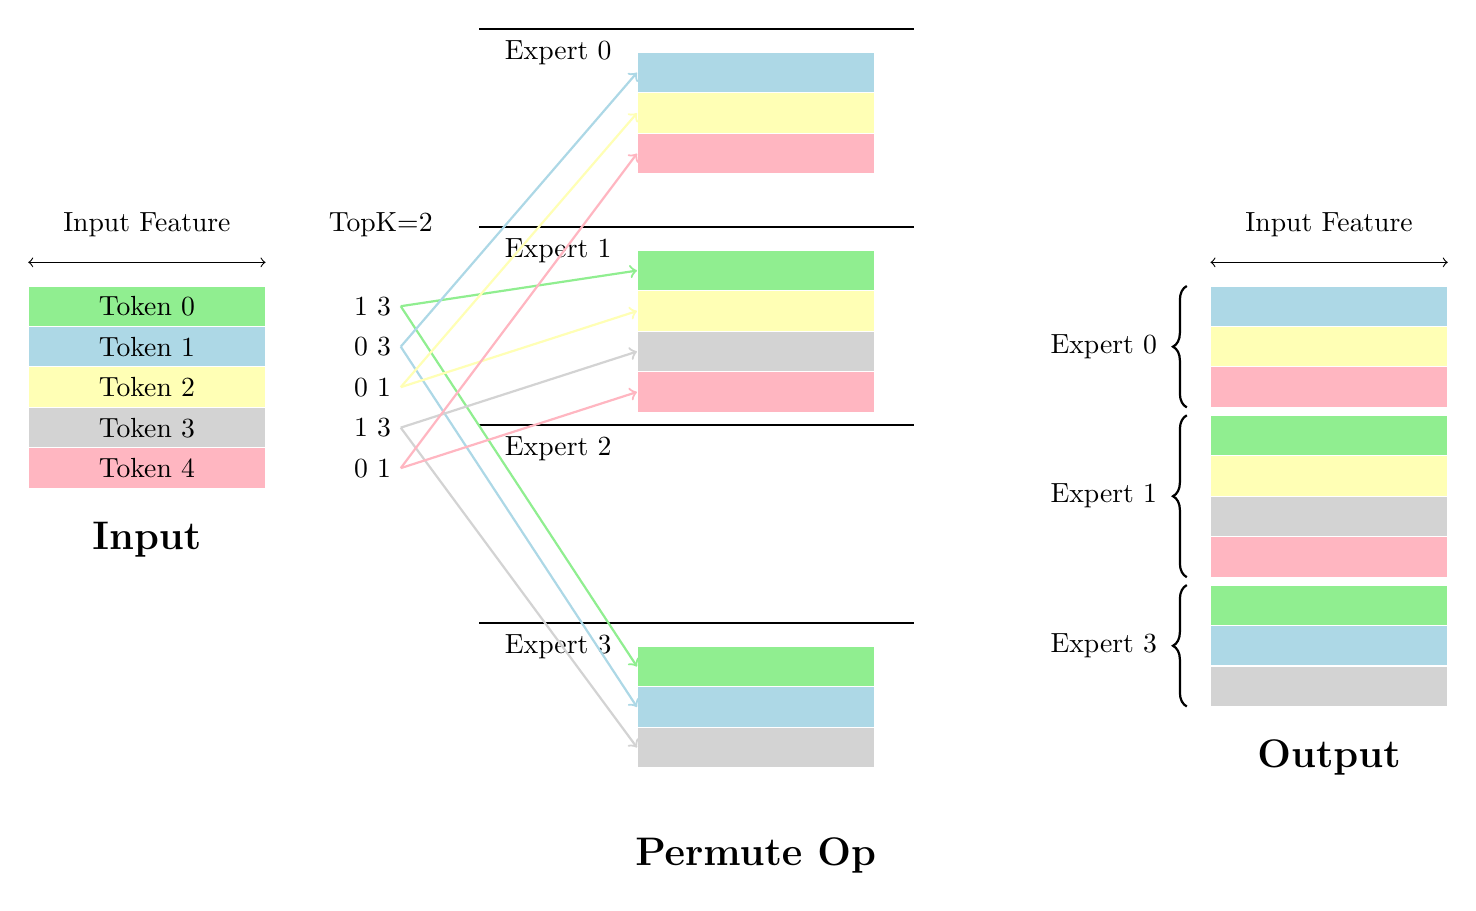
\begin{tikzpicture}[
    token/.style={rectangle, minimum width=3cm, minimum height=0.5cm},
    expert/.style={rectangle, minimum width=3cm, minimum height=2cm},
    output/.style={rectangle, minimum width=0.8cm, minimum height=0.4cm}
]

% 输入tokens
\node[token, fill=color1] (token0) {Token 0};
\node[token, fill=color2, below=0.0cm of token0] (token1) {Token 1};
\node[token, fill=color3, below=0.0cm of token1] (token2) {Token 2};
\node[token, fill=color4, below=0.0cm of token2] (token3) {Token 3};
\node[token, fill=color5, below=0.0cm of token3] (token4) {Token 4};

% Input标签
\node[below=0.3cm of token4] (input_label) {\Large \textbf{Input}};

% Input Feature标签
\node[above=0.5cm of token0] (input_feature_label) {Input Feature};
\draw[<->] ([yshift=0.3cm]token0.north west) -- ([yshift=0.3cm]token0.north east);

% TopK=2标签和数字
\node[right=1cm of input_feature_label] (topk_label) {TopK=2};
\node[right=1cm of token0] (numbers0) {1 3};
\node[right=1cm of token1] (numbers1) {0 3};
\node[right=1cm of token2] (numbers2) {0 1};
\node[right=1cm of token3] (numbers3) {1 3};
\node[right=1cm of token4] (numbers4) {0 1};

% 专家模块
\node[expert, above right=2cm and 3cm of numbers2] (expert0) {};
\node[expert, below=0.5cm of expert0] (expert1) {};
\node[expert, below=0.5cm of expert1] (expert2) {};
\node[expert, below=0.5cm of expert2] (expert3) {};

% 填充专家模块
\node[token, fill=color2, below=0.0cm of expert0.north]  (expert0_token1) {};
\node[token, fill=color3, below=0.0cm of expert0_token1] (expert0_token2) {};
\node[token, fill=color5, below=0.0cm of expert0_token2] (expert0_token3) {};

\node[token, fill=color1, below=0.0cm of expert1.north]  (expert1_token1) {};
\node[token, fill=color3, below=0.0cm of expert1_token1] (expert1_token2) {};
\node[token, fill=color4, below=0.0cm of expert1_token2] (expert1_token3) {};
\node[token, fill=color5, below=0.0cm of expert1_token3] (expert1_token4) {};

\node[token, fill=color1, below=0.0cm of expert3.north]  (expert3_token1) {};
\node[token, fill=color2, below=0.0cm of expert3_token1] (expert3_token2) {};
\node[token, fill=color4, below=0.0cm of expert3_token2] (expert3_token3) {};

% 专家标签
\node[left=0.2cm of expert0.north west] (expert0_label) {Expert 0};
\draw[thick] ([yshift=0.3cm, xshift=-2cm]expert0.north west) -- ([yshift=0.3cm, xshift=0.5cm]expert0.north east);
\node[left=0.2cm of expert1.north west] (expert1_label) {Expert 1};
\draw[thick] ([yshift=0.3cm, xshift=-2cm]expert1.north west) -- ([yshift=0.3cm, xshift=0.5cm]expert1.north east);
\node[left=0.2cm of expert2.north west] (expert2_label) {Expert 2};
\draw[thick] ([yshift=0.3cm, xshift=-2cm]expert2.north west) -- ([yshift=0.3cm, xshift=0.5cm]expert2.north east);
\node[left=0.2cm of expert3.north west] (expert3_label) {Expert 3};
\draw[thick] ([yshift=0.3cm, xshift=-2cm]expert3.north west) -- ([yshift=0.3cm, xshift=0.5cm]expert3.north east);

% 连接线
\draw[->, thick, color1] (numbers0.east) -- (expert1_token1.west);
\draw[->, thick, color1] (numbers0.east) -- (expert3_token1.west);
\draw[->, thick, color2] (numbers1.east) -- (expert0_token1.west);
\draw[->, thick, color2] (numbers1.east) -- (expert3_token2.west);
\draw[->, thick, color3] (numbers2.east) -- (expert0_token2.west);
\draw[->, thick, color3] (numbers2.east) -- (expert1_token2.west);
\draw[->, thick, color4] (numbers3.east) -- (expert1_token3.west);
\draw[->, thick, color4] (numbers3.east) -- (expert3_token3.west);
\draw[->, thick, color5] (numbers4.east) -- (expert0_token3.west);
\draw[->, thick, color5] (numbers4.east) -- (expert1_token4.west);

% 输出部分
\node[token, fill=color2, right=12cm of token0] (out0_0) {};
\node[token, fill=color3, below=0.0cm of out0_0] (out0_1) {};
\node[token, fill=color5, below=0.0cm of out0_1] (out0_2) {};

\node[token, fill=color1, below=0.1cm of out0_2] (out1_0) {};
\node[token, fill=color3, below=0.0cm of out1_0] (out1_1) {};
\node[token, fill=color4, below=0.0cm of out1_1] (out1_2) {};
\node[token, fill=color5, below=0.0cm of out1_2] (out1_3) {};

\node[token, fill=color1, below=0.1cm of out1_3] (out3_0) {};
\node[token, fill=color2, below=0.0cm of out3_0] (out3_1) {};
\node[token, fill=color4, below=0.0cm of out3_1] (out3_2) {};

% 大括号和输出标签
\node[below=0.3cm of out3_2] (output_label) {\Large \textbf{Output}};
\node[above=0.5cm of out0_0] (output_feature_label) {Input Feature};
\draw[<->] ([yshift=0.3cm]out0_0.north west) -- ([yshift=0.3cm]out0_0.north east);

% 大括号
\draw[thick, decorate, decoration={brace, amplitude=5pt}] 
    ([xshift=-0.3cm]out0_2.south west) -- ([xshift=-0.3cm]out0_0.north west) node[midway,xshift=-3em]{Expert 0};
\draw[thick, decorate, decoration={brace, amplitude=5pt}] 
    ([xshift=-0.3cm]out1_3.south west) -- ([xshift=-0.3cm]out1_0.north west) node[midway,xshift=-3em]{Expert 1};
\draw[thick, decorate, decoration={brace, amplitude=5pt}] 
    ([xshift=-0.3cm]out3_2.south west) -- ([xshift=-0.3cm]out3_0.north west) node[midway,xshift=-3em]{Expert 3};

% Permute Op标签
\node[below=0.3cm of expert3] (permute_label) {\Large \textbf{Permute Op}};

\end{tikzpicture}
\end{document}